\documentclass[10pt]{article}
\usepackage[margin=0.9in]{geometry}
\usepackage[T1]{fontenc}
\usepackage{lmodern}
\usepackage{amsmath,amssymb}
\usepackage{booktabs,tabularx,multirow}
\usepackage{graphicx}
\usepackage{enumitem}
\usepackage{xcolor}
\usepackage[hidelinks]{hyperref}
\usepackage{algorithm}
\usepackage{algpseudocode}
\usepackage{caption}
\captionsetup{font=small,labelfont=bf}
\setlist{nosep,leftmargin=*}
\newcommand{\OR}{\mathrm{OR}}

\title{\textbf{Feeling Understood Is Not Feeling Ownership:}\\
\large Survey, Interaction-Log, and Microsimulation Evidence from the CoAuthor Dataset}
\author{Exploratory secondary analysis\\
\small Draft of 2026-10-09 \quad Code: \url{https://github.com/yeona-lee-researcher/coauthor-ownership-analysis}}
\date{}

\begin{document}
\maketitle

\begin{abstract}
\noindent
Does feeling that an AI writing assistant understands one's intent go together with feeling that the text is one's own?
We linked CoAuthor metadata and post-session surveys (1,407 sessions with at least one AI request; 61 writer IDs), decomposed ratings into writer means and within-writer deviations, and fit cumulative-logit GEEs with writer-clustered errors.
The hypothesized positive within-writer association between perceived understanding and ownership was not supported ($\OR=0.847$, 95\% CI [0.660, 1.086]), whereas understanding was strongly associated with reported ideation help ($\OR=3.396$ [2.761, 4.176]) and human share of inserted text with ownership ($\OR=1.327$ per 10 pp [1.130, 1.559]).
We then replayed all 1,447 keystroke-level logs with per-character provenance, reproducing the metadata's human share within 1 pp in 99.9\% of sessions and its selection counts exactly.
In the logs, 6.8\% of requests were never answered, and within a writer, a higher unanswered rate was associated with lower perceived understanding ($\OR=0.770$ per 10 pp [0.687, 0.862]), suggesting that ``understanding'' ratings partly reflect system availability.
Requests followed typing after a median of 0.4\,s; only 2.1\% followed $\geq$10\,s of inactivity.
A semi-Markov microsimulation of writing, pausing, and request outcomes, validated on held-out writers and on writers' later sessions, showed that writer-specific parameters predict the same writer's future sessions better than a population model (+0.068 nats/event [0.041, 0.106]; 35 of 39 writers), i.e., writers have stable interaction styles.
Preliminary coding of 23 contrastive comments found useful help with low ownership and intent mismatch with high ownership.
We argue that ideation support, availability, and ownership should be evaluated separately, and propose \emph{role alignment} as a follow-up question. All findings are observational.
\end{abstract}

\section{Introduction}
What users value in co-creative writing may not be only the quality of the final text, but whether the text still carries \emph{their} intent: which direction they chose, which suggestions they accepted, and how they revised them.
If ``good AI use'' is defined by usage volume or output fluency alone, the experience of exploring with AI while remaining the author of one's work is invisible.

Our starting motivation is respect for the individual's own intent and values in human--AI collaboration, related to autonomy in self-determination theory~\cite{ryan2000sdt}.
CoAuthor~\cite{lee2022coauthor} contains no validated measures of authenticity, personality, intrinsic motivation, or well-being, so we restrict the survey question to three post-session ratings: \emph{the system understood what I was trying to write} (perceived understanding, $U$), \emph{the suggestions helped me come up with new ideas} (ideation help, $I$), and \emph{I feel like the story/essay is mine} (ownership, $O$).
Prior work shows that AI-generated text can lower perceived ownership even when users still declare authorship~\cite{draxler2024ghostwriter}, motivating us to treat ownership as distinct from both helpfulness and the amount of text typed by the human.

Because the same writers completed many sessions (median 9, range 1--89), we separate \textbf{between-writer} questions (do writers who generally feel understood report more ownership?) from \textbf{within-writer} questions (in sessions where the same person felt more understood than usual, did they also feel more ownership?)~\cite{curran2011disaggregation}.
Because post-session ratings say nothing about \emph{how} a session unfolded, we also replay the raw interaction logs to ask what the process looks like, whether it explains the ratings, and whether individuals have stable interaction styles that a generative model can capture.

\paragraph{Hypotheses and questions.} H1--H3 were fixed after inspecting the data structure but before the first model run (not preregistered); E1--E4 and the simulation were specified after the survey results and qualitative coding and are exploratory.
\begin{itemize}
  \item \textbf{H1 (primary).} Within-writer $U$ is positively associated with $O$, adjusting for human share, prompt, and model setting.
  \item \textbf{H2.} Within-writer $U$ is positively associated with $I$.\quad
        \textbf{H3.} The within-writer $I$--$O$ association is more positive when within-writer $U$ is higher.
  \item \textbf{RQ4 (qualitative).} Where $U$ and $O$ agree or diverge, how do writers describe support, mismatch, choice, and role?
  \item \textbf{E1--E4 (logs).} Is system availability associated with $U$ (E1)? Is revising AI text associated with $O$ (E2)? Do requests follow pauses (E3)? How much does the writer type after each request outcome (E4)?
  \item \textbf{S (simulation).} Can a descriptive process model reproduce sessions of unseen writers, and do writer-specific parameters improve prediction of a writer's later sessions?
\end{itemize}
H1 is the single primary test; H2--H3 are Holm-corrected as one family.

\section{Data}
We downloaded the four official sheets (creative/argumentative metadata and surveys) as XLSX and used the 1,447 public \texttt{.jsonl} interaction logs. Sessions were linked one-to-one by trimmed session ID within genre; worker IDs agreed for all linked sessions (Table~\ref{tab:flow}).

\begin{table}[h]
\centering\small
\caption{Sample flow for the survey analysis.}\label{tab:flow}
\begin{tabular}{lrl}
\toprule
Step & $n$ & Note \\
\midrule
Metadata sessions & 1,445 & creative 830, argumentative 615 \\
Survey rows & 1,458 & creative 833, argumentative 625 \\
\quad excess duplicate survey rows & $-3$ & latest response kept (earliest as sensitivity) \\
\quad surveys with no metadata match & $-11$ & not imputed or fuzzy-matched \\
Linked sessions & 1,444 & 1 metadata session had no survey \\
\quad zero-query sessions & $-37$ & observed non-use, not missing data \\
\textbf{Analysis sample} & \textbf{1,407} & creative 823, argumentative 584; 61 writer IDs \\
\bottomrule
\end{tabular}
\end{table}

\paragraph{Variables.} $U$, $I$, $O$: 1--7 ratings. $H$: metadata \texttt{written\_by\_human}, entered per 10 pp. CoAuthor's Table 3 describes this as the share of \emph{final} text written by writers; at the session level, our replay shows that it matches the human share of \emph{inserted} characters (within 1 pp in 99.9\% of sessions, vs.\ 43\% for the final-text share), although the two definitions give nearly the same mean (73.0\% vs.\ 72.7\%; the paper reports 72.6\%). Prompt (20 levels) enters as fixed effects; model setting is the genre-specific high/low decoding configuration. Session duration is not treated as time pressure, as the CoAuthor timer indicated a minimum, not a deadline.

\paragraph{Discrepancies to resolve.} CoAuthor reports 63 writers (58 creative, 49 argumentative), whereas the public metadata contain 61 unique IDs (57 and 47). Section~5.2.2 of the paper describes ownership as a 5-point Likert scale, whereas Appendix~C lists the other items as 7-point and the downloaded ownership responses range 1--7. We used the observed coding and flag both for confirmation with the dataset authors.

\section{Method}
\subsection{Survey models}
For writer $i$ and session $j$, $\bar U_i = n_i^{-1}\sum_j U_{ij}$ and $U^W_{ij} = U_{ij}-\bar U_i$ (likewise for $H$). We fit
\begin{equation}
\operatorname{logit}\Pr(O_{ij}>k)=\alpha_k+\beta_W U^W_{ij}+\beta_B\bar U_i+\gamma_W\tfrac{H^W_{ij}}{10}+\gamma_B\tfrac{\bar H_i}{10}+\delta_{p(ij)}+\theta_C R^C_{ij}+\theta_A R^A_{ij},\quad k=1,\dots,6,
\end{equation}
by stacking cumulative indicators $\mathbb{1}(O_{ij}>k)$ and solving the working-independence ordinal GEE score, with a writer-clustered sandwich covariance, $G/(G{-}1)$ correction, and $t_{G-1}$ intervals ($G{=}61$).
$\exp(\beta_W)$ is a common cumulative odds ratio, not a probability ratio or causal effect.
The estimator was implemented in NumPy/SciPy and checked numerically (analytic vs.\ finite-difference gradient $1.0\times10^{-7}$; intercept-only model reproduces observed cumulative proportions to $8.5\times10^{-10}$; Frisch--Waugh--Lovell check of the linear FE coefficient to $10^{-16}$).
All 547 reported parameters reproduce to $10^{-5}$ across two software stacks (Python 3.12/SciPy 1.17 and 3.14/1.18), except three prompt coefficients in the $O>3$ threshold model that are not identified because of quasi-complete separation ($|\hat\beta|\approx 29$); these are nuisance terms.

\paragraph{Sensitivity analyses} (added after initial results; all reported): equal total weight per writer; session order; usage and duration; additional ratings (ideation, fluency); zero-query sessions included; earliest duplicate response; genre-specific fits; threshold-specific models $O>k$; a linear writer fixed-effects model with a 500-resample writer bootstrap.

\subsection{Log replay and process features}
Each log was replayed delta by delta, labeling every character as prompt, human, or AI. Sessions were segmented into episodes:
\textbf{W} (writing burst; user text events separated by $<$10\,s),
\textbf{P} (inactivity $\geq$10\,s),
\textbf{QA}/\textbf{QR} (suggestions shown and one accepted / none accepted),
and \textbf{QN} (request with no suggestions shown before the writer resumed).
Edge cases found during validation were handled explicitly: suggestions displayed after the writer had resumed typing (88 episodes; the earlier request is marked \emph{answered late} and not counted as unanswered), re-opened suggestion lists (45), and selections from a panel left open while typing.
Pauses are observed inactivity, not ``being stuck.''
Session features include the unanswered-request rate, median latency, mean number of suggestions shown, acceptance rate, and the \emph{AI revision rate} (share of inserted AI characters later deleted by the writer).
E1 and E2 add within/between-writer splits of these features to the ordinal GEE (outcomes $U$ and $O$). E3 is descriptive by design: bursts are separated only by pauses, so ``pause $\rightarrow$ more writing'' is structural and a regression on it would be tautological. E4 regresses human characters typed in the 30/60\,s after a request on its outcome with writer fixed effects, excluding windows censored by session end.

\subsection{Process model and microsimulation}
Let $s_t\in\{\mathrm{W},\mathrm{P},\mathrm{QA},\mathrm{QR},\mathrm{QN}\}$. For writer $i$ in genre $g$, with $n_{iab}$ observed $a\!\to\!b$ transitions,
\begin{align}
\pi_{iab} &= \frac{n_{iab}+\kappa\,\pi^{\mathrm{pop}}_{gab}}{n_{ia\cdot}+\kappa}, \qquad
\boldsymbol\pi^{(\text{session})}_{a\cdot}\sim \mathrm{Dirichlet}(\alpha\,\boldsymbol\pi_{ia\cdot}),\\
(\Delta t, h, c)\mid s_t{=}k &\sim \lambda_{ik}\hat F_{ik}+(1-\lambda_{ik})\hat F_{gk},\quad \lambda_{ik}=\frac{N_{ik}}{N_{ik}+\kappa},\qquad
\Pr(\text{stop}\mid \text{bin } b) = \frac{e_{ib}+\kappa_h h_{gb}}{u_{ib}+\kappa_h},
\end{align}
where $(\Delta t, h, c)$ are an episode's duration (including the short gap before it), human characters, and AI characters, drawn jointly by resampling the writer's or the genre's episodes; the stopping hazard uses 30-s bins of elapsed time.
The session-level Dirichlet captures session-to-session variation within a writer; $\alpha$ is scored by sequential P\'olya-urn predictive likelihood.
$\kappa$, $\kappa_h$, and $\alpha$ are tuned on an inner split of training data only.
The model is descriptive: it does not infer latent states, personality, or motivation.

\begin{algorithm}[h]
\small
\caption{Validation and use of the microsimulation (seed 20261009; 100 replicates per session)}
\begin{algorithmic}[1]
\State \textbf{A. Unseen writers.} Split writers into 5 folds. For each fold: tune $\alpha$ on an inner writer split of the training writers; fit M0 (iid tokens), M1 (first-order), M1+S (M1 with session Dirichlet) on training writers; score held-out log-likelihood; simulate each held-out session.
\State \textbf{B. Later sessions of known writers.} For writers with $\ge$6 sessions, hold out the later half of each writer's sessions (by time). Tune $\kappa,\kappa_h,\alpha$ on the earlier vs.\ later halves of the \emph{training} sessions. Compare population, writer ($\kappa$), and full (writer + stopping + session) models by held-out log-likelihood (writer bootstrap) and predictive checks.
\State \textbf{Checks.} For each session: is the observed summary inside the simulated 90\% interval? Absolute error of the simulated median; KS distance of pooled distributions.
\State \textbf{C. Variance share.} Fit the full model on all data; simulate 200 sessions per writer$\times$genre; compare simulated with observed intraclass correlations.
\State \textbf{D. Scenario.} With common random numbers, move each row's QN probability to QA/QR in proportion; report changes. Model-implied, not causal.
\end{algorithmic}
\end{algorithm}

\subsection{Qualitative contrast sampling}
Cells crossed $U\le3$ vs.\ $\ge6$, $O\le3$ vs.\ $\ge6$, and genre (8 cells; ratings 4--5 excluded). In each cell, sessions with a non-empty comment were shuffled (seed 20261009) and up to 3 selected, at most 1 per writer, yielding 23 sessions from 16 writers.
Coding was not blind, was produced by a single AI-assisted coder, and has not yet been reviewed by a human coder; we report patterns, not prevalences, and do not claim a reflexive thematic analysis~\cite{braun2021}. Comments mostly answer an ``improvement'' prompt, which biases toward criticism.

\section{Results}
\subsection{Survey descriptives and hypothesis tests}
Ownership was concentrated at the top of the scale (565 sessions at 7, 406 at 6). Means (SD): ownership 5.87 (1.23) creative vs.\ 5.94 (1.16) argumentative; understanding 5.52 (1.52) vs.\ 5.39 (1.63); ideation help 5.47 (1.71) vs.\ 5.06 (1.89); human share 73.2\% vs.\ 71.0\%. Pooled Spearman correlations with ownership were small (understanding .058, ideation .105, human share .281); the last is consistent with the Pearson correlation of 0.3 between ownership and the fraction of text written by writers reported by CoAuthor (Section~5.2.2).

\begin{table}[h]
\centering\small
\caption{Main conditional associations (cumulative odds ratios, writer-clustered 95\% CI).}\label{tab:main}
\begin{tabular}{llccl}
\toprule
Outcome & Predictor & OR & 95\% CI & $p$ \\
\midrule
Ownership & $U^W$ (H1) & 0.847 & [0.660, 1.086] & .187 \\
Ownership & $\bar U$ (between) & 2.356 & [1.565, 3.547] & $<$.001 \\
Ownership & $H^W$ (+10 pp) & 1.327 & [1.130, 1.559] & $<$.001 \\
Ideation help & $U^W$ (H2) & 3.396 & [2.761, 4.176] & Holm $<$.001 \\
Ownership & $U^W\times I^W$ (H3) & 0.940 & [0.876, 1.009] & Holm .087 \\
\bottomrule
\end{tabular}
\end{table}

\textbf{H1 was not supported}; the point estimate is below 1 and the interval includes 1, and we do not reinterpret it as ``understanding lowers ownership.''
\textbf{H2 was supported} as an association between two post-hoc ratings (shared response style and item overlap are plausible contributors). \textbf{H3 was not supported.}
No sensitivity specification produced a positive within-writer association (Table~\ref{tab:sens}). Under equal-writer weighting the between-writer OR fell from 2.356 to 1.374 [0.978, 1.932], so it depends on heavily participating writers. The linear writer-FE estimate was $-0.094$ points [$-0.226$, 0.037] (bootstrap [$-0.205$, 0.028]). Threshold-specific ORs declined from 1.016 ($O>3$) to 0.741 ($O>6$), suggesting threshold heterogeneity that the proportional-odds summary may hide.

\begin{table}[h]
\centering\small
\caption{Within-writer understanding $\to$ ownership across specifications.}\label{tab:sens}
\begin{tabular}{lcc@{\qquad}lcc}
\toprule
Specification & OR & 95\% CI & Specification & OR & 95\% CI\\
\midrule
Primary & 0.847 & [0.660, 1.086] & + fluency rating & 0.832 & [0.644, 1.074]\\
Equal writer weight & 0.854 & [0.735, 0.992] & Incl.\ zero-query & 0.847 & [0.659, 1.088]\\
+ session order & 0.852 & [0.663, 1.094] & Earliest duplicate & 0.847 & [0.660, 1.086]\\
+ usage, duration & 0.839 & [0.651, 1.082] & Creative only & 0.927 & [0.693, 1.240]\\
+ ideation rating & 0.919 & [0.768, 1.101] & Argumentative only & 0.741 & [0.572, 0.959]\\
\bottomrule
\end{tabular}
\end{table}

\subsection{Qualitative contrasts}
\begin{table}[h]
\centering\small
\caption{Illustrative contrastive cases (paraphrased, not quoted). $U/I/O$ on 1--7; $H$ = human share.}\label{tab:qual}
\begin{tabularx}{\linewidth}{@{}l c c X X@{}}
\toprule
Pattern & $U/I/O$ & $H$ & Writer's account (paraphrase) & What it supports \\
\midrule
Useful support, low ownership & 7/7/2 & 39\% & Used many suggestions; described self as closer to an editor than a writer. & Helpfulness, role, and ownership are distinct. \\
Mismatch, high ownership & 3/2/7 & 89\% & AI's creative suggestions did not fit the intended direction. & Mismatch and ownership can co-occur. \\
Unstuck, low ownership & 6/6/3 & 87\% & Got stuck midway; AI's new direction let them continue. & Help and low ownership coexist despite high human share. \\
Deliberate delegation & 7/7/3 & 15\% & Let the AI set topic and direction to test the system. & Low ownership need not mean unwanted loss of agency. \\
Questions scaffold expression & 2/5/6 & 78\% & Criticized latency but liked AI questions that made them write. & A low $U$ may reflect availability, not all support. \\
Choosing among options & 6/5/6 & 66\% & Could choose the story's direction among several suggestions. & Candidate for measuring control directly. \\
\bottomrule
\end{tabularx}
\end{table}
Across cases, low understanding ratings often co-occurred with complaints about service (no suggestions, latency) rather than semantic mismatch. E1 tests this pattern in the logs.

\subsection{What the logs show}
\paragraph{Replay validity.} Replayed duration matched metadata \texttt{time} (ratio 0.999--1.002); replayed human share of inserted characters matched \texttt{written\_by\_human} within 1 pp in 99.9\% of sessions (vs.\ 43\% if computed on the final text); replayed selections matched \texttt{num\_selected} in 100\%. Metadata \texttt{num\_query} counts answered requests (91.6\% exact), so it omits unanswered ones.

\paragraph{Process descriptives.} The 1,445 linked logs contain 44,326 episodes. Of 18,089 requests, 1,231 (6.8\%) were never answered, affecting 505 sessions; the mean unanswered rate was 4.1\% in creative and 11.8\% in argumentative sessions. Median latency was 2.0\,s; on average 4.3 (creative) and 3.8 (argumentative) of the 5 requested suggestions were shown. Writers accepted a suggestion in 76\% / 71\% of displays, and later deleted a median of 0.7\% / 2.9\% of inserted AI characters (means 5.9\% / 9.5\%).

\begin{table}[h]
\centering\small
\caption{Log-linked exploratory models (E1, E2: ordinal GEE with prompt, model setting, and $H$ split; writer-clustered 95\% CI).}\label{tab:logs}
\begin{tabular}{lllcc}
\toprule
& Outcome & Within-writer predictor & OR & 95\% CI \\
\midrule
E1 & Understanding & Unanswered rate (+10 pp) & \textbf{0.770} & [0.687, 0.862] \\
 & & Mean suggestions shown (+1) & \textbf{1.353} & [1.102, 1.663] \\
 & & log median latency & 1.367 & [0.600, 3.114] \\
 & & Human share (+10 pp) & \textbf{0.690} & [0.570, 0.836] \\
E2 & Ownership & AI revision rate (+10 pp) & 0.996 & [0.843, 1.176] \\
 & & Human share (+10 pp) & \textbf{1.290} & [1.122, 1.483] \\
\bottomrule
\end{tabular}
\end{table}

\paragraph{E1: availability and understanding.} In sessions where the same writer experienced more unanswered requests or fewer displayed suggestions than usual, they rated understanding lower (Table~\ref{tab:logs}). The corresponding between-writer terms were imprecise. Writers also rated understanding lower in sessions where they typed a larger share themselves.
\paragraph{E2: revising AI text.} Deleting more of the inserted AI text was not associated with ownership ($n=1{,}388$ sessions with at least one acceptance); ownership tracked the human share of inserted text instead. This agrees with CoAuthor's observation that the number of edit events was not meaningfully correlated with ownership ($r=0.1$), here with a provenance-based measure and within-writer adjustment.
\paragraph{E3: pauses and requests.} Requests followed the last writing event after a median of 0.41\,s (IQR 0.20--1.04; 90th percentile 2.7\,s). Only 2.1\% [1.2, 4.0] of requests followed $\geq$10\,s of inactivity (0.9\% for $\geq$20\,s, 0.5\% for $\geq$30\,s; writer-bootstrap CIs). Conversely, 7.9\% [5.7, 9.9] of $\geq$10-s pauses after writing ended in a request (10.9\% for $\geq$30\,s). In these logs, requesting a suggestion is mostly an in-flow action rather than a response to a long stall.
\paragraph{E4: writing after a request.} In the 60\,s after a request, writers typed 15.4 [4.1, 26.8] more characters after an unanswered request and 10.0 [1.3, 18.6] more after a rejected one than after an accepted one (writer FE). This is expected mechanically, since accepted text substitutes for typing.

\subsection{Microsimulation}
Population transitions were similar across genres: after a writing burst the next unit was an accepted request (creative 61\%, argumentative 53\%), a pause (20\% / 24\%), a rejected request (16\% / 17\%), or an unanswered request (3\% / 7\%); unanswered requests were followed by another unanswered request 16\% / 13\% of the time (repeated failures).

\begin{table}[h]
\centering\small
\caption{Validation of the process model. Coverage = share of observed sessions inside the simulated 90\% interval (nominal 0.90). Q episodes include requests, late displays, and reopened lists. M0 knows token frequencies but not their order.}\label{tab:sim}
\begin{tabular}{lccccc}
\toprule
& Log-lik/event & \multicolumn{4}{c}{Coverage} \\
\cmidrule(lr){3-6}
Model & (held out) & Q episodes & Accepted & Human share & Duration \\
\midrule
\multicolumn{6}{l}{\emph{A. Unseen writers (5-fold by writer)}} \\
M0 iid tokens & $-1.272$ & .680 & .683 & .673 & .856 \\
M1 first-order & $-0.804$ & .552 & .580 & .549 & .851 \\
M1 + session heterogeneity & $\mathbf{-0.745}$ & .636 & .730 & .659 & .866 \\
\midrule
\multicolumn{6}{l}{\emph{B. Later sessions of known writers (39 writers, 707 held-out sessions)}} \\
Population & --- & .584 & .583 & .542 & .888 \\
Writer ($\kappa{=}20$) & $+0.068$ vs.\ pop. & .733 & .757 & .737 & .884 \\
Writer + stopping + session ($\kappa_h{=}5,\alpha{=}10$) & $+0.044$ vs.\ writer & \textbf{.809} & \textbf{.809} & \textbf{.771} & \textbf{.926} \\
\bottomrule
\end{tabular}
\end{table}

\begin{figure}[h]
\centering
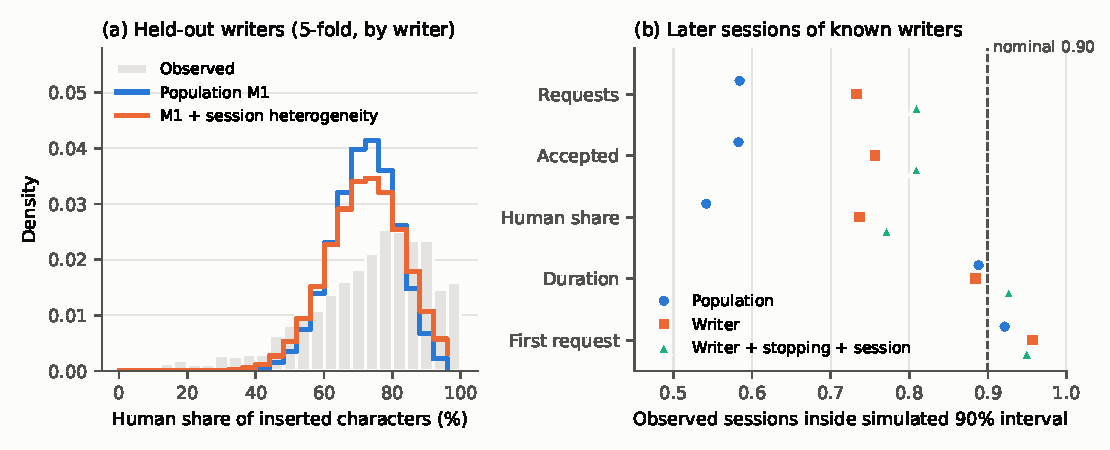
\includegraphics[width=\linewidth]{fig_simulation.pdf}
\caption{(a) Distribution of the human share of inserted characters for held-out writers: observed vs.\ simulated. Simulated sessions are too concentrated and miss the high tail (sessions with little AI use). (b) 90\% predictive-interval coverage for writers' later sessions; writer-specific parameters move coverage toward nominal.}\label{fig:sim}
\end{figure}

\paragraph{A. Unseen writers.} The first-order model predicted held-out writers' event sequences much better than a model that knows only token frequencies ($-0.804$ vs.\ $-1.272$ nats/event): the \emph{order} of actions carries information, e.g., an accepted suggestion was followed by a writing burst 86--87\% of the time. Session heterogeneity improved prediction further ($-0.745$); because its P\'olya-urn score updates on transitions already observed in the same session, this gain means that patterns emerging within a session are informative, not that a writer's style is known before the session starts. Part of the sequential regularity is induced by segmentation (consecutive writing events form one burst). All models reproduced mean session summaries (e.g., human share 72.2\% simulated vs.\ 73.0\% observed) but were under-dispersed (simulated SD of human share 11.3 vs.\ 18.2; Figure~\ref{fig:sim}a). M0's similar coverage reflects noise, not a better description of the process.

\paragraph{B. Individual interaction styles.} Writer-specific parameters predicted the same writers' later sessions better than the population model: +0.068 nats/event [0.041, 0.106], positive for 35 of 39 writers. Session heterogeneity added +0.044 [0.018, 0.070] and writer-specific stopping +0.010 [0.005, 0.017]. Compared with the population model, the full model reduced the absolute error of the predicted human share by 4.96 pp [2.74, 7.20], of requests by 1.93 [0.93, 2.88], and of accepted suggestions by 1.44 [0.76, 2.11]; coverage approached but did not reach nominal (Figure~\ref{fig:sim}b). Coverage of session duration was already adequate (.888 population, .926 full). The log-score gain is not an accuracy percentage; it is the improvement in the log-probability assigned to the actions that occurred.

\paragraph{C. How much is the writer?} Observed intraclass correlations were high (human share .56 creative / .70 argumentative; Q episodes .56 / .84). This in-sample check (the model is fit to all data, unlike B) shows that the full model reproduces much of the clustering in creative writing (.54, .50) but under-reproduces it in argumentative writing (.57, .65), and fails for duration (.15 / .06 vs.\ .61 / .57): overall session lengths are reproduced, but not the tendency of particular writers to write consistently long or short sessions. ICCs describe recurring differences between writers, which may reflect skill, task choice, strategy, or habit, not personality.

\paragraph{D. Scenario (model-implied, not causal).} Replacing the never-answered share of QN episodes (90\% creative, 97\% argumentative; the rest were answered late) with accepted or rejected displays in each row's observed ratio implies +0.53 [0.40, 0.66] accepted suggestions per session, $-1.32$ pp [$-1.60$, $-1.03$] human share of inserted characters, and $-0.16$ Q episodes. A lower human share here means more AI-inserted characters, not less human direction or creativity. The scenario quantifies the scale of availability failures under the model; it is not an intervention effect.

\section{Discussion}
\paragraph{Ideation help, availability, and ownership are different outcomes.}
Within a writer, feeling understood tracked feeling helped, not feeling ownership. The logs add that ``understanding'' ratings also track whether the system responded at all, so a single satisfaction-style score would mix model quality, service availability, and ideation support. Ownership instead tracked the human share of inserted text, not whether writers revised AI text afterwards.

\paragraph{Stable individual styles, situational variation.}
This project began from the question of whether individuals bring an ``internal component'' to their interaction with AI. The process model gives an observable answer: request, acceptance, and writing patterns are writer-specific and predictive of the same writer's future sessions, yet sessions also vary substantially around each writer's style. These are behavioral regularities, not measures of personality or motivation.

\paragraph{Role alignment as a follow-up question.}
Cases suggest that low ownership is not necessarily a bad outcome: a writer who chose to act as an editor may report low ownership accurately. A design goal may be to ensure that the \emph{experienced role matches the desired role}, not to maximize ownership. This hypothesis emerged from the analysis and has not been tested.

\paragraph{Limitations.}
Single-item, same-time self-reports cannot identify causal order; human share may itself be a consequence of the collaboration, so the adjusted $\beta_W$ is not a total effect. Ratings are ceiling-heavy and proportional odds may not hold. Sixty-one clusters limit between-writer and interaction estimates. E1--E4 and the simulation were specified post hoc. The process model is first-order with resampled episode contents; it remains under-dispersed (coverage .77--.81 for counts in B), misses the high tail of human share, and under-individualizes stopping. The data reflect paid crowdworkers using GPT-3 in 2021. Qualitative coding is preliminary and awaits human review; the 63/61 writer and 5/7-point discrepancies remain unresolved. No claims are made about authenticity, motivation, or mental health.

\section{Future Work}
\begin{enumerate}
  \item \textbf{Richer process model.} Add session-level emission heterogeneity and a session-level (not per-unit) stopping model; condition transitions on document position and recent acceptance history; test higher-order or hidden-state models only if they improve held-out likelihood, without naming hidden states as traits.
  \item \textbf{Link process to experience.} Within-writer models of $O$ and $I$ on process trajectories (e.g., runs of consecutive acceptances, where in the text AI content lands).
  \item \textbf{Experiment.} A $2\times2$ design crossing an intent-confirmation interface (goal/perspective check vs.\ time-matched neutral preparation) with time budget (tight vs.\ generous), measuring ownership (primary), ideation help, perceived control, blind-rated creativity, and desired vs.\ experienced role; preregistered, intention-to-treat, with power analysis by simulation from the fitted process model rather than from observational ORs.
\end{enumerate}

\paragraph{Reproducibility.}
\texttt{python run\_pipeline.py --input <xlsx> --logs <coauthor-v1.0>} runs linkage, survey models, hash-checked qualitative join, log replay, process models, microsimulation, and figures in under a minute. \texttt{verify\_results.py} compares a rerun with \texttt{reference\_results/}; 9 unit tests cover data guards and replay provenance. A fresh clone with a freshly downloaded workbook, pinned packages, and Python 3.11 reproduced all survey parameters, the process-model estimates to $2\times10^{-8}$, and the simulation report byte for byte.

\small
\begin{thebibliography}{9}
\bibitem{lee2022coauthor} M.~Lee, P.~Liang, and Q.~Yang. CoAuthor: Designing a human--AI collaborative writing dataset for exploring language model capabilities. In \emph{Proceedings of the 2022 CHI Conference on Human Factors in Computing Systems}, 2022. \url{https://doi.org/10.1145/3491102.3502030}. Data: \url{https://coauthor.stanford.edu/}
\bibitem{draxler2024ghostwriter} F.~Draxler et al. The AI ghostwriter effect: When users do not perceive ownership of AI-generated text but self-declare as authors. \emph{ACM Transactions on Computer-Human Interaction}, 31(2), Article 25, 1--40, 2024. \url{https://doi.org/10.1145/3637875}
\bibitem{curran2011disaggregation} P.~J.~Curran and D.~J.~Bauer. The disaggregation of within-person and between-person effects in longitudinal models of change. \emph{Annual Review of Psychology}, 62:583--619, 2011. \url{https://doi.org/10.1146/annurev.psych.093008.100356}
\bibitem{ryan2000sdt} R.~M.~Ryan and E.~L.~Deci. Self-determination theory and the facilitation of intrinsic motivation, social development, and well-being. \emph{American Psychologist}, 55(1):68--78, 2000. \url{https://doi.org/10.1037/0003-066X.55.1.68}
\bibitem{braun2021} V.~Braun and V.~Clarke. Can I use TA? Should I use TA? Should I not use TA? Comparing reflexive thematic analysis and other pattern-based qualitative analytic approaches. \emph{Counselling and Psychotherapy Research}, 21(1):37--47, 2021. \url{https://doi.org/10.1002/capr.12360}
\end{thebibliography}
\end{document}
